\documentclass{article}
\usepackage[english]{babel}
\usepackage[utf8]{inputenc}
\usepackage[T1]{fontenc}
\usepackage{graphicx}
\usepackage{caption}
\usepackage{subcaption}
\usepackage{float}
\usepackage{wrapfig}
\usepackage{setspace}
\usepackage{cite}
\usepackage{url}
\usepackage{color}
\definecolor{linkcol}{rgb}{0,0,0.4}
\definecolor{citecol}{rgb}{0.5,0,0}
\usepackage[pagebackref,hyperindex=true]{hyperref}
\hypersetup{colorlinks=true,linkcolor=linkcol,citecolor=citecol,urlcolor=linkcol}

\begin{document}

\begin{titlepage}
\begin{center}
  \hfill
  \vspace{3.0cm}

  {\huge \textsc{IO Operations for wavepackets with HDF5 Interface in C++\\[10pt]
  }}
  ~\\[20pt]

  {\huge{Bachelor Thesis}}\\[2.5cm]

  {\emph{written by}}\\
  Florian Frei
  \\[0.6cm]
  {\emph{supervised by}}\\
  Dr. Vasile Gr\u{a}dinaru\\
  {\emph{and}}\\
  Prof. Dr. Ralf Hiptmair
  \\[2.5cm]

  Seminar for Applied Mathematics\\
  ETH Zurich
  \\[0.5cm]
  \emph{{Spring semester 2016}}
\end{center}
\end{titlepage}



\tableofcontents
\clearpage

\section{Introduction}
This thesis is about the continuation of the C++ implementation \cite{libwaveblocks} and allows a comparison to the Python implementation \cite{waveblocksnd}. The already existing framework is sufficient to generate simulations of different kind of Hagedorn wavepackets. The data produced is written in HDF5 binary format whereas the data from the C++ implementation is not easily comparable to the generated data from python. The writing process in the C++ implementation is currently done by using an extern project \cite{eigen3-hdf5}. The new implementation for writing binary HDF format in C++ will be explained in this thesis and also the new implementation allows easy comparison between Python and C++. It also incorporates a testing file which takes two HDF binary data files as arguments and compares the coinciding data. The testing file uses the well-known GoogleTest interface\cite{googletest}.

\section{HDF5 C++ Interface}
\subsection{Overview}
From the documentation we can conclude that the C++ interface is just a nice wrapper of the C interface. The corresponding classes and wrappers are shown in the following table:
\begin{figure}[!h]
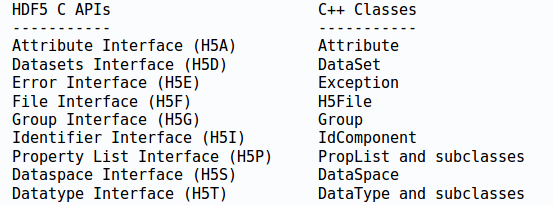
\includegraphics[width=1.2\textwidth]{c_vs_cpp.png}
\caption{Relation of the C und C++ library}
\end{figure}
The hierarchy of these classes is depicted in the following diagramm:
\begin{figure}[!h]
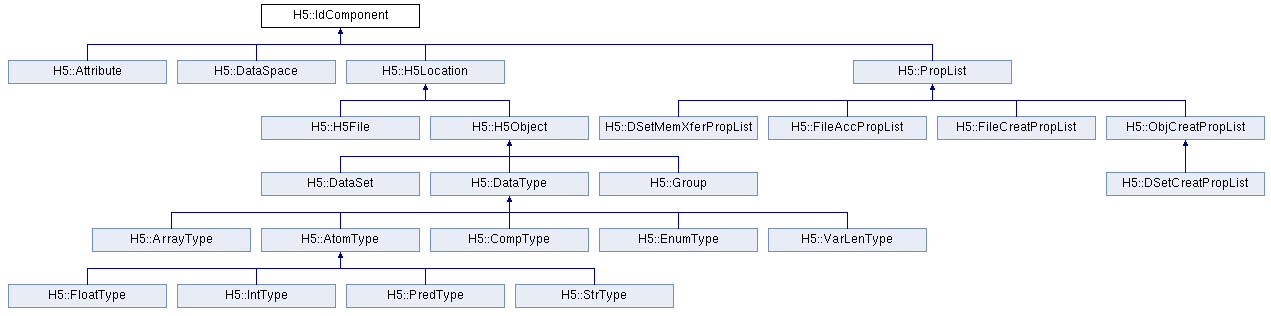
\includegraphics[width=1.2\textwidth]{inheritance_diagramm.png}
\caption{Inheritance diagram of IdComponent}
\end{figure}
For our purposes we need to save a Hagedorn wave packet in every time step which consists of matrices and vectors. For these we need a DataSpace which allows us to write matrices and vectors in a time-dimension. In our case the time-dimension is arbitrarily chosen depending on the kind of the simulation. As such we need a DSetCreatePropList which is used to describe properties such as chunk-dimension for matrices used in our case for time-dimension. Attribute are used to save additional information such as the used time-step $\delta t$ in the simulation. For constructing a HDF5 binary file we need to use the File class which simply uses a string argument as the filename. For neatness we want to have a intern structure for our data. For this we use the Group class which is very similar to the file system and its folders for structuring. Last but not least we need the defined DataSet class to store our Eigen-matrices within and to write these we have to use the HDF5 DataTypes.

\subsection{Intern used data-types}
Often we make function calls with arguments to the HDF5 library. These arguments have to be of an intern data type. 
\subsubsection{hsize$\_$t}
\subsubsection{H5std$\_$string}
\subsection{DataType}
\subsection{DataSpace}
\subsection{DataSet}
\subsection{Attribute}
\subsection{DSetCreatePropList}
\subsection{Group}
\subsection{File}

\section{Eigen Interface}

\section{HDF5 Writer template}

\section{Datatest with GoogleTest Framework}
\subsection{Initialization}
\subsection{Testfissure}
\subsection{Testclass including HDF5 Interface}


%\nocite{*}


\bibliographystyle{plain}
\bibliography{references,wp,own}

\end{document}
